 \documentclass[a4paper,fleqn]{cas-dc}

%%%Author definitions
\def\tsc#1{\csdef{#1}{\textsc{\lowercase{#1}}\xspace}}
\tsc{WGM}
\tsc{QE}
\tsc{EP}
\tsc{PMS}
\tsc{BEC}
\tsc{DE}
%%%

\usepackage[square,numbers,sort&compress,comma]{natbib}

\usepackage{amsmath}
\usepackage{amssymb}
\usepackage{diagbox}
\usepackage{caption}
\usepackage{graphicx}
\usepackage{latexsym}
\usepackage{times}
\usepackage[pagewise]{lineno}
\graphicspath{{figures/}}
\usepackage{color, colortbl}
\usepackage{chemformula}
\usepackage{xcolor}
\definecolor{Gray}{gray}{0.9}
\newcommand{\highlight}[1]{%
  \colorbox{Gray}{$\displaystyle#1$}}
\usepackage{color, colortbl}
\usepackage{chemformula}
\usepackage{xcolor}
\usepackage{adjustbox}
\usepackage{mathrsfs}
\usepackage{booktabs}
\usepackage{hyperref}
\usepackage{lipsum}

\emergencystretch = 0 pt
\pretolerance = 150
\tolerance = 250
\hbadness = 150
\hfuzz = 0 pt
\vfuzz = 0 pt

\usepackage{color}
\definecolor{color-strings}{rgb}{0,0,0.5}
\definecolor{color-keywords}{rgb}{0.6,0,0}
\definecolor{color-comments}{rgb}{0,0.5,0}
\definecolor{color-background}{rgb}{0.99,0.99,0.99}
\definecolor{color-numbers}{rgb}{0.7,0.7,0.7}
\definecolor{color-classes}{rgb}{0.2,0.3,0.4}

\usepackage{listings}
\lstdefinestyle{mystyle}{
	basicstyle=\ttm,
    backgroundcolor=\color{color-background},   
    commentstyle=\color{color-comments},
    keywordstyle=\color{color-keywords}\bfseries,
    numberstyle=\tiny\color{color-numbers},
    stringstyle=\color{color-strings},
    basicstyle=\linespread{0.8}\ttfamily\scriptsize,
    breakatwhitespace=false,         
    breaklines=true,                 
    captionpos=b,                    
    keepspaces=true,                 
    numbers=left,                    
    numbersep=5pt,                  
    showspaces=false,                
    showstringspaces=false,
    showtabs=false,                  
    tabsize=2,
    emph={pykitPIV, Particle, ParticleSpecs, FlowField, FlowFieldSpecs, Image, ImageSpecs, Motion, MotionSpecs, Postprocess, PIVDataset, PIVEnv, CameraAgent, Rewards, Cues, gymnasium, gym, Env},
    emphstyle=\bfseries\color{color-classes},
}

\lstset{style=mystyle} 

\newcommand{ \kamila}[1]{\color{blue}{Kamila: #1} \color{black}}
\newcommand{ \todump}[1]{\color{olive}{#1} \color{black}}
\usepackage[normalem]{ulem}

\begin{document}

\shorttitle{\texttt{pykitPIV}: Rich and reproducible virtual training of machine learning algorithms in optical velocimetry}
\shortauthors{Zdyba\l{} et~al.}

\title [mode = title]{\texttt{pykitPIV}: Rich and reproducible virtual training of machine learning algorithms in optical velocimetry}

\author[EMPA]{Kamila Zdyba\l{}*}
\ead{kamila.zdybal@gmail.com}

\author[EMPA]{Claudio Mucignat}
\author[EMPA]{Stefan Kunz}
\author[EMPA]{Ivan Lunati}

\address[EMPA]{Laboratory for Computational Engineering, Swiss Federal Laboratories for Materials Science and Technology, Empa, Dübendorf, Switzerland}

\begin{abstract}
In recent years, machine learning (ML) has become an increasingly integral part of experimental fluid dynamics. 
This calls for new tools that can emulate real wind tunnel experiments and generate high-quality training data and testbeds for ML model development.
Here, we present \texttt{pykitPIV}, a Python library that provides rich and reproducible virtual environments for training ML algorithms in optical velocimetry. The generated synthetic datasets and environments mimic those coming from particle image velocimetry (PIV) and background-oriented Schlieren (BOS) experimental techniques. 
The library integrates with various ML algorithms, such as convolutional neural networks, variational approaches, active learning, and reinforcement learning. This library gives the user, or the ML agent, flexibility in selecting various parameters that would normally be available in an experimental setting, such as seeding density, properties of the laser plane, camera exposure, particle loss, or experimental noise. We also provide an atlas of challenging synthetic velocity fields from analytic formulations (both compressible and incompressible) where the effects of particle drift and diffusion in stationary isotropic turbulence can also be added using the simplified Langevin model.
With \texttt{pykitPIV}, ML agents have the freedom to interact with the virtual experiment, can assimilate data from real experiment, and can be trained to perform a variety of tasks using diverse sensory cues and rewards. Our goal is to support the current trends in the velocimetry community for faster and more accurate real-time experimental inference, moving the field towards autonomous experimentation and building robust models from experimental data.
\end{abstract}

\begin{keywords}
particle image velocimetry; flow estimation; convolutional neural networks; machine learning; reinforcement learning; Python
\end{keywords}

\maketitle

\section{Motivation and significance\label{sec:introduction}}

% INTRODUCE CNNs FOR OPTICAL FLOW IN GENERAL, NOT JUST FOR PIV
The last decade has seen advances in training convolutional neural networks (CNNs) for optical flow estimation, \textit{i.e.}, predicting motion information from recorded image frames separated by a short time interval. To date, numerous network architectures have been developed that are highly specialized for this application. These include various implementations of FlowNets \citep{dosovitskiy2015flownet, ilg2017flownet, hui2018liteflownet}, the spatial pyramid network (SPyNet) \cite{ranjan2017optical}, the pyramid, warping, and cost-volume network (PWC-Net) \cite{sun2018pwc}, and, more recently, the recurrent all-pairs field transforms (RAFT) \cite{teed2020raft}. In addition, the introduction of iterative residual refinement (IRR) \cite{hur2019iterative} allowed for a significant reduction in the number of trainable parameters thanks to weight sharing at several levels of successively upscaled image resolution.

% EXPERIMENTAL F. D. SPECIFICALLY CAN PROFIT FROM THOSE CNNs 
Experimental fluid dynamics can especially profit from those architectures. Specifically, particle image velocimetry (PIV) and background-oriented Schlieren (BOS) are optical techniques used to visualize flow patterns with high precision. Their main goal is to predict flow targets, such as displacement fields, velocity components, or vorticity, either from paired snapshots of illuminated tracer particles injected into the flow (in PIV) or from recorded deformations of the dotted background image (in BOS). Recently, RAFT-PIV \cite{lagemann2021deep} and lightweight image-matching architecture (LIMA) \citep{manickathan2023lightweight} were proposed as versions of CNNs that are optimized for inference from velocimetry experiments. The successes of RAFT-PIV and LIMA have been demonstrated on a number of classic experimental fluid dynamics settings such as flow behind a cylinder, boundary layer flow, or convective flow of a hot air plume \cite{mucignat2023lightweight}. The advancements to these architectures are continually being made in the context of PIV \citep{yu2021lightpivnet, fan2023deep, choi2023deep, shan2024lightweight, elrefaie2024site} with the goal to replace and outperform state-of-the-art PIV post-processing in the future. Currently, the main precedence that has motivated the need for those networks is that they can be trained on GPUs within the matter of hours and then ported to laboratory hardware to make flow predictions in real-time, parallel to experimental measurements.
% THE SUCCESS OF THOSE CNNs IN F. D. OPENS UP NEW AVENUES OF ML RESEARCH
Moreover, the advances made in optical flow architectures open up new avenues of research and allow for new machine learning (ML) use-cases to emerge that have not been possible before. In that sense, CNNs can become a gateway to various other ML algorithms such as variational approaches, active learning, or reinforcement learning (RL). This can allow the experimental community to develop new applications such as autonomous experimentation, data assimilation and digital twinning, building models from experimental data, and enhanced flow control.

% THERE' STILL WORK TO BE DONE...
% TO IMPROVE CNNs
% BUT ALSO NOW THAT THOSE AVENUES HAVE BEEN OPENED UP, WE CAN DO SO MUCH MORE...
To advance the performance and applications of CNN architectures in experimental fluid dynamics, a number of research questions will have to be addressed in the future:
\begin{enumerate}
\item How rich should the training dataset be to remain applicable in a practical range of experimental settings?
\item At which challenging experimental settings do the current CNNs fail and why?
\item Can we assimilate data collected on-the-fly with the experiment, \textit{e.g.}, using active learning procedure?
\item Can variational/generative approaches be used to create improved training datasets whose distribution more closely matches the distribution of a given experimental setting?
\item Can we then accomplish transfer learning using a pre-trained inference model?
\item As ML for PIV post-processing becomes widely used, how do we make sure that training settings are reproducible and can be easily shared between research groups?
\end{enumerate}

% OUR SOFTWARE HELPS TO DO THAT WORK.
To help researchers answer those questions and move the field towards unexplored research directions, in this paper, we present \texttt{pykitPIV} (\textbf{Py}thon \textbf{ki}nematic \textbf{t}raining for \textbf{PIV}), a Python library that provides virtual velocimetry environments and ready-to-use ML integrations. In that sense, our library can serve as a ``virtual wind tunnel''. At its core, \texttt{pykitPIV} exploits the kinematic relationship between two consecutive time frames in the wind tunnel \cite{manickathan2022kinematic}. Given any velocity field, tracer particles are advected from one time frame to the next using a second-order accurate numerical scheme. Synthetic dataset used to train CNNs are scarce and often do not exploit challenging flow scenarios. \texttt{pykitPIV} addresses this gap and allows for rich experimental conditions to be generated and presented to ML algorithms as batches of training data. The associated post-processing targets (\textit{e.g.}, displacement fields) establish the ground truth for ML algorithms. This is in contrast to raw experimental data which lacks the ground truth. Finally, \texttt{pykitPIV} contains a standalone ML module which integrates with the virtual wind tunnel and gives the ML agents flexibility in interacting with the experimental settings. We also provide a variety of sensory cues and rewards for training RL agents. This paves the way towards development of autonomous experimentation in the future.

\begin{figure*}[t]
\centering
\vspace{-0.4 in}
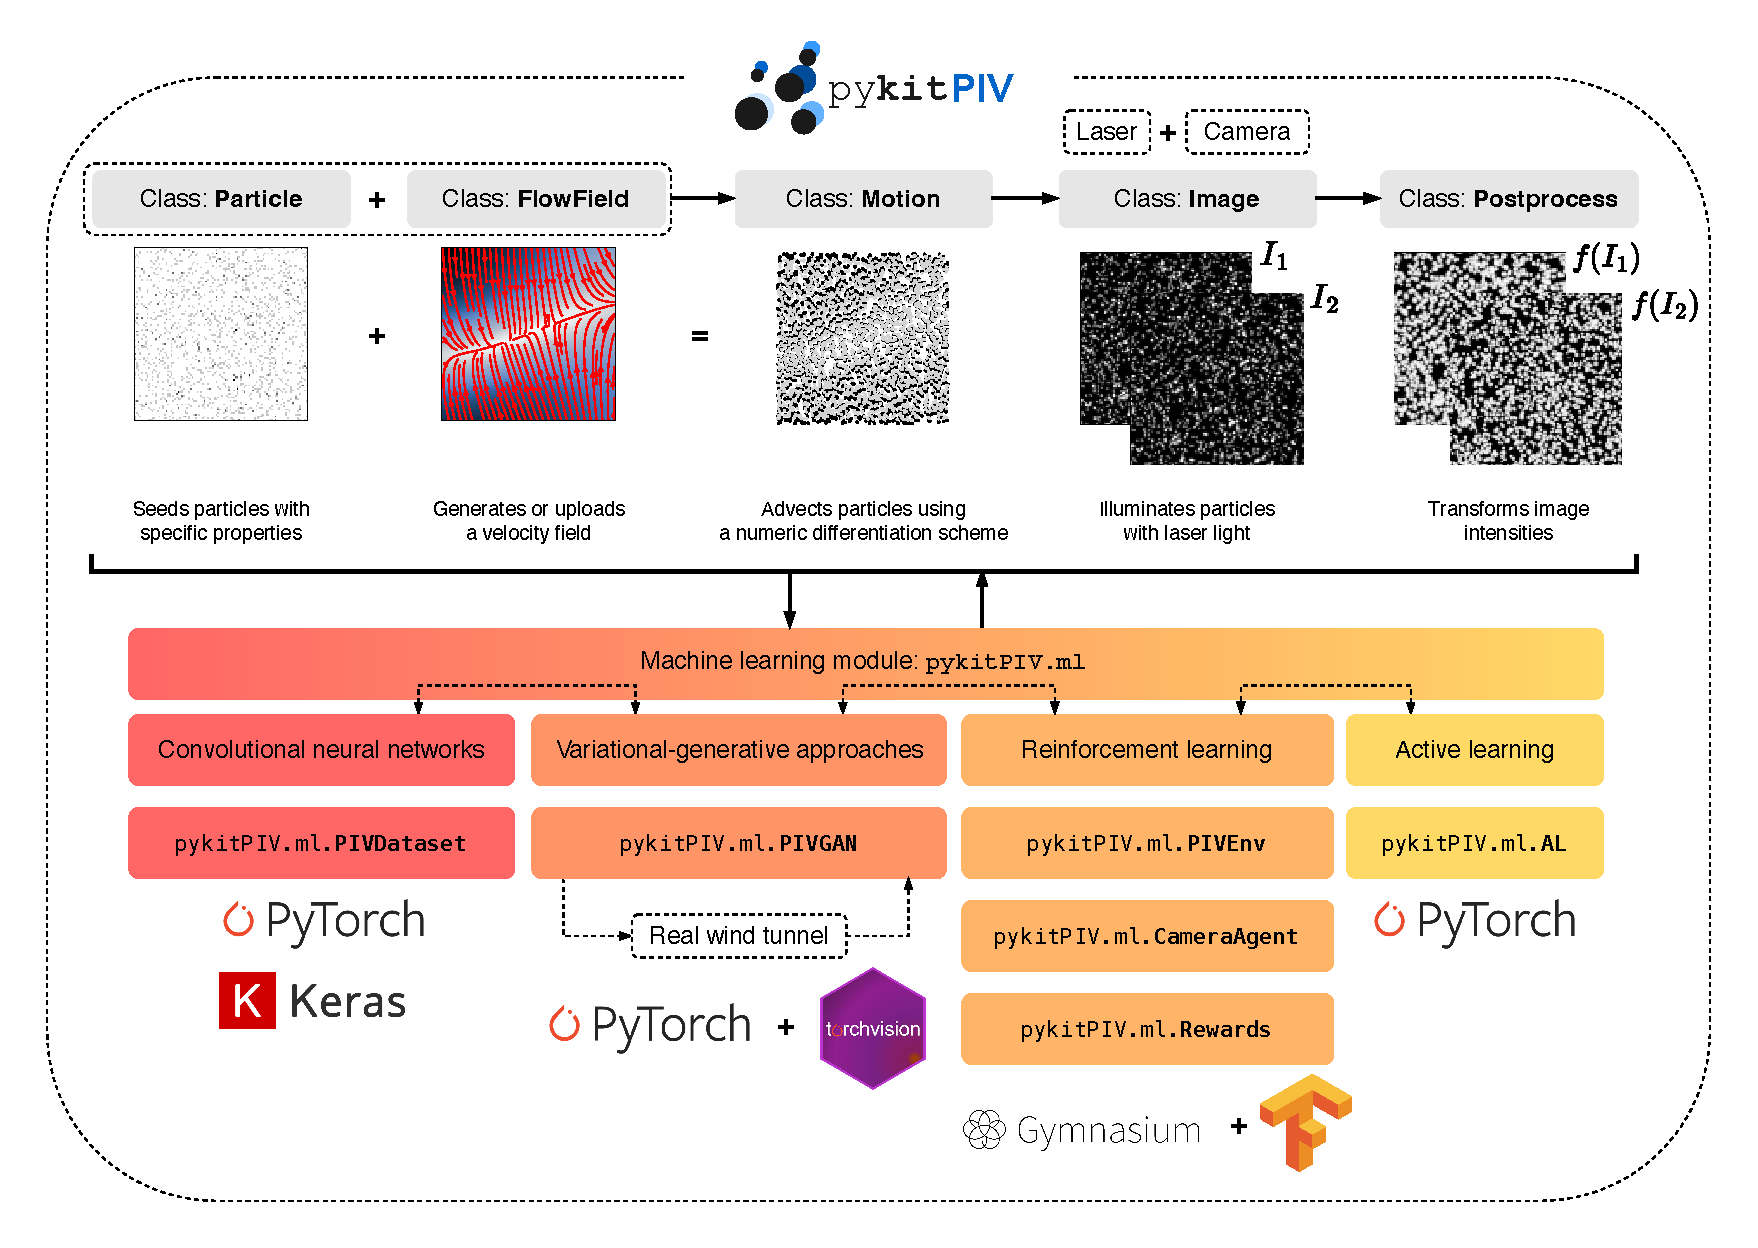
\includegraphics[width=\textwidth]{pykitPIV-modules.pdf}
\vspace{10 pt}
\caption{\footnotesize Order of using the five main \texttt{pykitPIV} classes that act as a virtual experimental setup with which the ML module, \texttt{pykitPIV.ml}, interacts. At each stage of synthetic virtual experimentation, the user, or the ML agent, has freedom in selecting various parameters that would normally be available in an experimental setting such as the seeding density, properties of the laser plane, camera exposure, particle loss, or experimental noise. The various ML components can also communicate and enrich each other. We note that \texttt{pykitPIV} uses sequential colormaps by Crameri et al. \cite{crameri2020misuse}.}
\label{fig:pykitPIV-overview}
\end{figure*}

\section{Software description} \label{sec:software}

\subsection{Software architecture}

The functionalities of \texttt{pykitPIV} that provide the ``virtual wind tunnel'' are organized in five classes: \texttt{Particle}, \texttt{FlowField}, \texttt{Motion}, \texttt{Image}, and \texttt{Postprocess}. Each class has a clear-cut role in generating synthetic image pairs and the corresponding flow targets. Beyond the five main classes, we provide a dedicated ML module, \texttt{pykitPIV.ml}, which contains wrappers and integrations to various ML algorithms. The main power of \texttt{pykitPIV}'s architecture is that the ML module can interact with the five main classes. Fig.~\ref{fig:pykitPIV-overview} illustrates the hierarchy of using \texttt{pykitPIV}'s classes and presents the scope of the ML module.

\subsection{Software functionalities}

Synthetic PIV/BOS image generation can only be a crude approximation of the real experimental flow conditions. For this reason, our goal in creating \texttt{pykitPIV} is to capture various complexities of the real-world experimental settings. In essence, the five main classes of \texttt{pykitPIV} (as per Fig.~\ref{fig:pykitPIV-overview}) provide a virtual optical velocimetry experimentation. They can generate paired image intensities, $I_1$ and $I_2$, separated by $\Delta t$ in time, and the corresponding displacement fields, $d\vec{\mathbf{s}} = [d \mathbf{x}, d\mathbf{y}]$, that have per-pixel resolution by construction. Moreover, experimental settings can be Monte-Carlo-generated and individual images within a training batch can span a range of conditions. At each stage of image generation, the user can fix random seeds to assure that data generation is fully reproducible. Below, we briefly describe what can be achieved in each class:
\begin{itemize}
\item The \texttt{Particle} class seeds the 2D flow domain with tracer particles. The user can steer the range of particle diameters and their standard deviation, the seeding density, or the average distances between particles. The initial particle positions are those appearing on snapshots $I_1$.
\item The \texttt{FlowField} class allows to generate the velocity field to be applied on the 2D domain. We implemented several methods to generate velocity fields, such as constant, random smooth, sinusoidal, checkered, Chebyshev polynomials, spherical harmonics, radial flows, and potential flows. This variety of velocity fields span cases with smooth and sharp velocity gradients, and compressible \textit{vs.} incompressible flows, and can help put ML algorithms to test. Atop any synthetic velocity field, the user can model the effect of particle drift and diffusion in isotropic turbulence using the simplified Langevin model (see \S12.6 in \cite{pope2001turbulent} for more information). The user also has the option of uploading an external velocity field, \textit{e.g.}, coming from a numerical simulation of Navier-Stokes equations or coming from a synthetic turbulence generator \citep{saad2017scalable, richards2018fast}. A selection of available flow fields is illustrated in Fig.~\ref{fig:velocity-fields}.
\item The \texttt{Motion} class applies the flow field to the particles. It uses the forward Euler or the Runge-Kutta 4th order numeric scheme to advect particles by the user-specified time separation, $\Delta t$. Velocity components in-between the grid points are interpolated with a regular grid interpolation. The main output of this class are particle positions that will appear on snapshots $I_2$, each paired with a respective snapshot $I_1$. The user can also steer the amount of particles lost between frame $I_1$ and $I_2$ due to out-of-laser-plane movement.
\item The \texttt{Image} class generates image intensities. It adds the reflected laser light to the generated PIV image pairs. The core functionality is to add a Gaussian intensity to each particle \citep{olsen2000out, rabault2017performing}. The user has a lot of flexibility in setting up the laser plane and camera properties. The \texttt{Image} class contains convenient functions for saving images to \texttt{.h5} files and for plotting or animating image pairs.
\item The \texttt{Postprocess} class contains functions that apply transformations to generated images, such as Gaussian noise, shot noise, and log-transformations.
\end{itemize}

\begin{figure}[t]
\centering
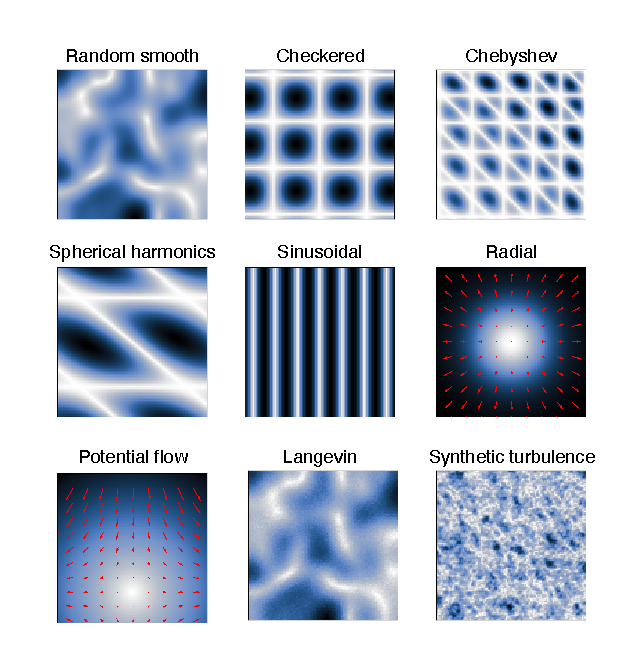
\includegraphics[width=8.5cm]{velocity-fields.pdf}
\caption{The types of 2D velocity fields that can be generated with the \texttt{FlowField} class. The user also has the option to upload an external velocity field, \textit{e.g.}, coming from synthetic turbulence \citep{saad2017scalable, richards2018fast} or turbulence databases \cite{perlman2007data}.}
\label{fig:velocity-fields}
\end{figure}

The ML module then provides classes and functionalities that integrate CNNs and RL with the ``virtual wind tunnel''. For example, we provide a RL environment (the \texttt{PIVEnv} class), the associated RL agent (the \texttt{CameraAgent} class) that uses deep double Q-learning \cite{van2016deep} with memory replay \cite{liu2018effects}, and a selection of rewards (the \texttt{Rewards} class) and sensory cues (the \texttt{Cues} class) that are applicable to fluid dynamics problems--see Table~\ref{tab:rewards-and-cues} for an overview.

\begin{table}[htbp]
  \centering
  \begin{tabular}{ll} 
    \toprule
    \textbf{Sensory cues} & \textbf{Rewards} \\
    \midrule[1.2pt]
    Vector field & Q-criterion \cite{jeong1995identification} \\
    Scalar field & Divergence \\
    Sampled vectors & Vorticity \\
    Divergence & Correlation \cite{lagemann2024challenges} \\
    Vorticity & Charbonier loss \cite{charbonnier1994two} \\
      & Structural similarity index measure \cite{wang2018occlusion} \\
      & Ternary census loss  \cite{zabih1994non} \\
      & Image frame consistency \cite{lagemann2024challenges} \\
      & Smoothness \cite{lagemann2024challenges} \\
    \bottomrule
  \end{tabular}
  \caption{A selection of sensory cues and rewards implemented in the ML module, \texttt{pykitPIV.ml} that can be readily used for RL agents using the \texttt{Cues} and the \texttt{Rewards} classes.}
  \label{tab:rewards-and-cues}
\end{table}

\section{Illustrative examples} \label{sec:examples}

\subsection{Porting with convolutional neural networks} \label{sec:example-CNN}

Here, we show how a synthetic PIV dataset can be generated and used to train LIMA \cite{manickathan2023lightweight}. For this, we use the class \texttt{PIVDataset} from the ML module which is a subclass of \texttt{torch.utils.data.Dataset} \cite{paszke2019pytorch}. The full tutorial can be accessed from the \href{https://pykitpiv.readthedocs.com}{software documentation}.

To create a diversity of samples in the training dataset, the user can randomize PIV parameters through two-element tuples that steer the minimum and maximum value for parameters such as particle diameters, seeding density, flow field features, camera exposure, or particle loss. The PIV image pairs tensor has shape $(N, 2, H, W)$, where $N$ is the batch size, $H$ is image height and $W$ is image width. The second dimension can be thought of as the number of channels and those correspond to $I_1$ and $I_2$, respectively. This is compatible with tensor shape accepted by convolutional layers implemented in PyTorch. Note that the whole batch of $N$ images can be generated all at once or can be optimized for memory and generated in mini-batches. Once the dataset has been saved, it can be loaded to the PyTorch data loader and passed to LIMA:
\lstset{language=Python}
\begin{lstlisting}
from pykitPIV.ml import PIVDataset

path = 'pykitPIV-dataset.h5'

PIV_data = PIVDataset(dataset=path)
\end{lstlisting}
With this, the user can inspect the data sample at a given index:
\lstset{language=Python}
\begin{lstlisting}
(I, target) = PIV_data[2]
\end{lstlisting}
or at multiple indices:
\lstset{language=Python}
\begin{lstlisting}
(I, target) = PIV_data[2:7]
\end{lstlisting}
The training dataset is then used to train the LIMA model. Fig.~\ref{fig:LIMA} shows an example inference of the challenging displacement field with small feature sizes and sharp displacement gradients. We note that thanks to its targeted architecture and parameters, LIMA achieves high accuracy and per-pixel spatial resolution.

\begin{figure}[t]
\centering
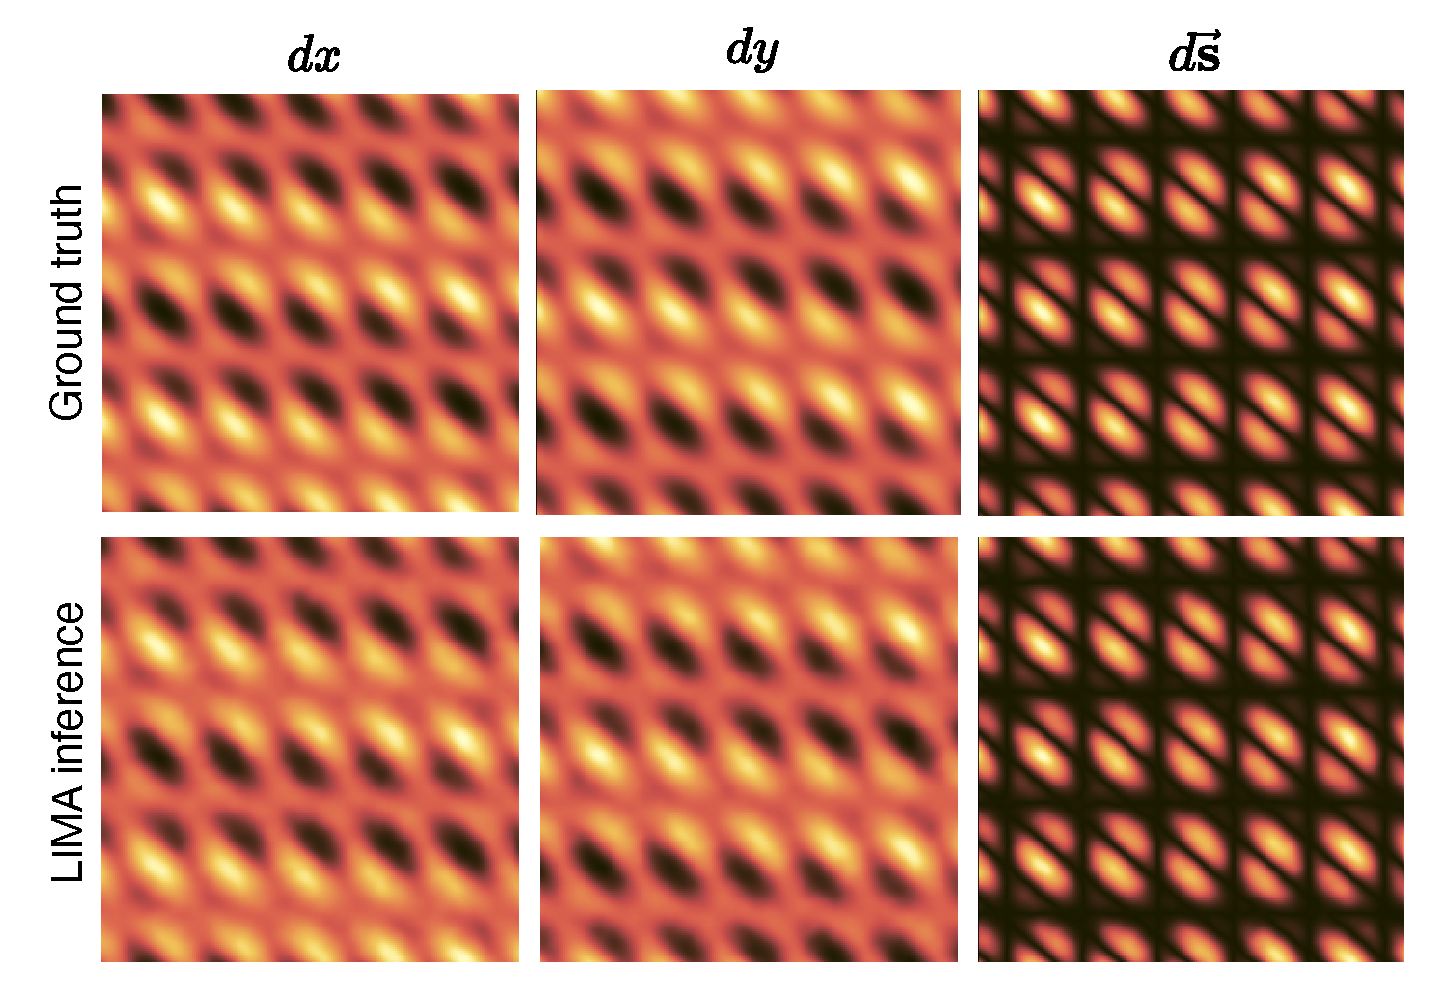
\includegraphics[width=8.5cm]{LIMA-inference.pdf}
\caption{Inference from the trained LIMA model on a challenging displacement field with small feature sizes. \kamila{This is my old training case, I will update it with the latest LIMA version after running new training on CSCS...}}
\label{fig:LIMA}
\end{figure}

\subsection{Reinforcement learning environments} \label{sec:example-RL}

Here, we demonstrate how \texttt{pykitPIV}'s functionalities can be used to train a RL agent to locate sources/sinks in a radial flow by moving a virtual camera over a 2D environment. 
This RL setup is presented in Fig.~\ref{fig:RL}a. The full tutorial can be accessed from the \href{https://pykitpiv.readthedocs.com}{software documentation}.

We assume that the camera only sees a portion of the virtual wind tunnel at a time, \textit{i.e.}, an interrogation window of 100px $\times$ 100px. Underneath each interrogation window are ground truth displacement fields, which result in respective PIV recordings. The RL agent then makes inference of the ground truth using the trained LIMA model from \S\ref{sec:example-CNN}. The sensory cues that the agent has available at each training step are 32 sampled displacement vectors at each interrogation window. Based on those cues, a divergence-based reward is computed as per the following equation:
\begin{equation} \label{eq:max-abs-div-reward}
R = \text{max} ( |\nabla \cdot d\vec{\mathbf{s}} | )
\end{equation}
To access this reward from \texttt{pykitPIV} the user can instantiate an object of the \texttt{Rewards} class and access one of the available rewards functions. Note that the rewards functions accept a custom transformation function that gives the user extra flexibility in how the final reward value is computed. The example for creating a reward as in Eq.~(\ref{eq:max-abs-div-reward}) is presented below.
\lstset{language=Python}
\begin{lstlisting}
from pykitPIV import Rewards
import numpy as np

velocity_field = ...

rewards = Rewards(verbose=True,
                  random_seed=None)
                  
def transformation(div):
    return np.max(np.abs(div))
    
R = rewards.divergence(velocity_field=velocity_field,
transformation=transformation)
\end{lstlisting}

\begin{figure*}[t]
\centering
\vspace{-0.4 in}
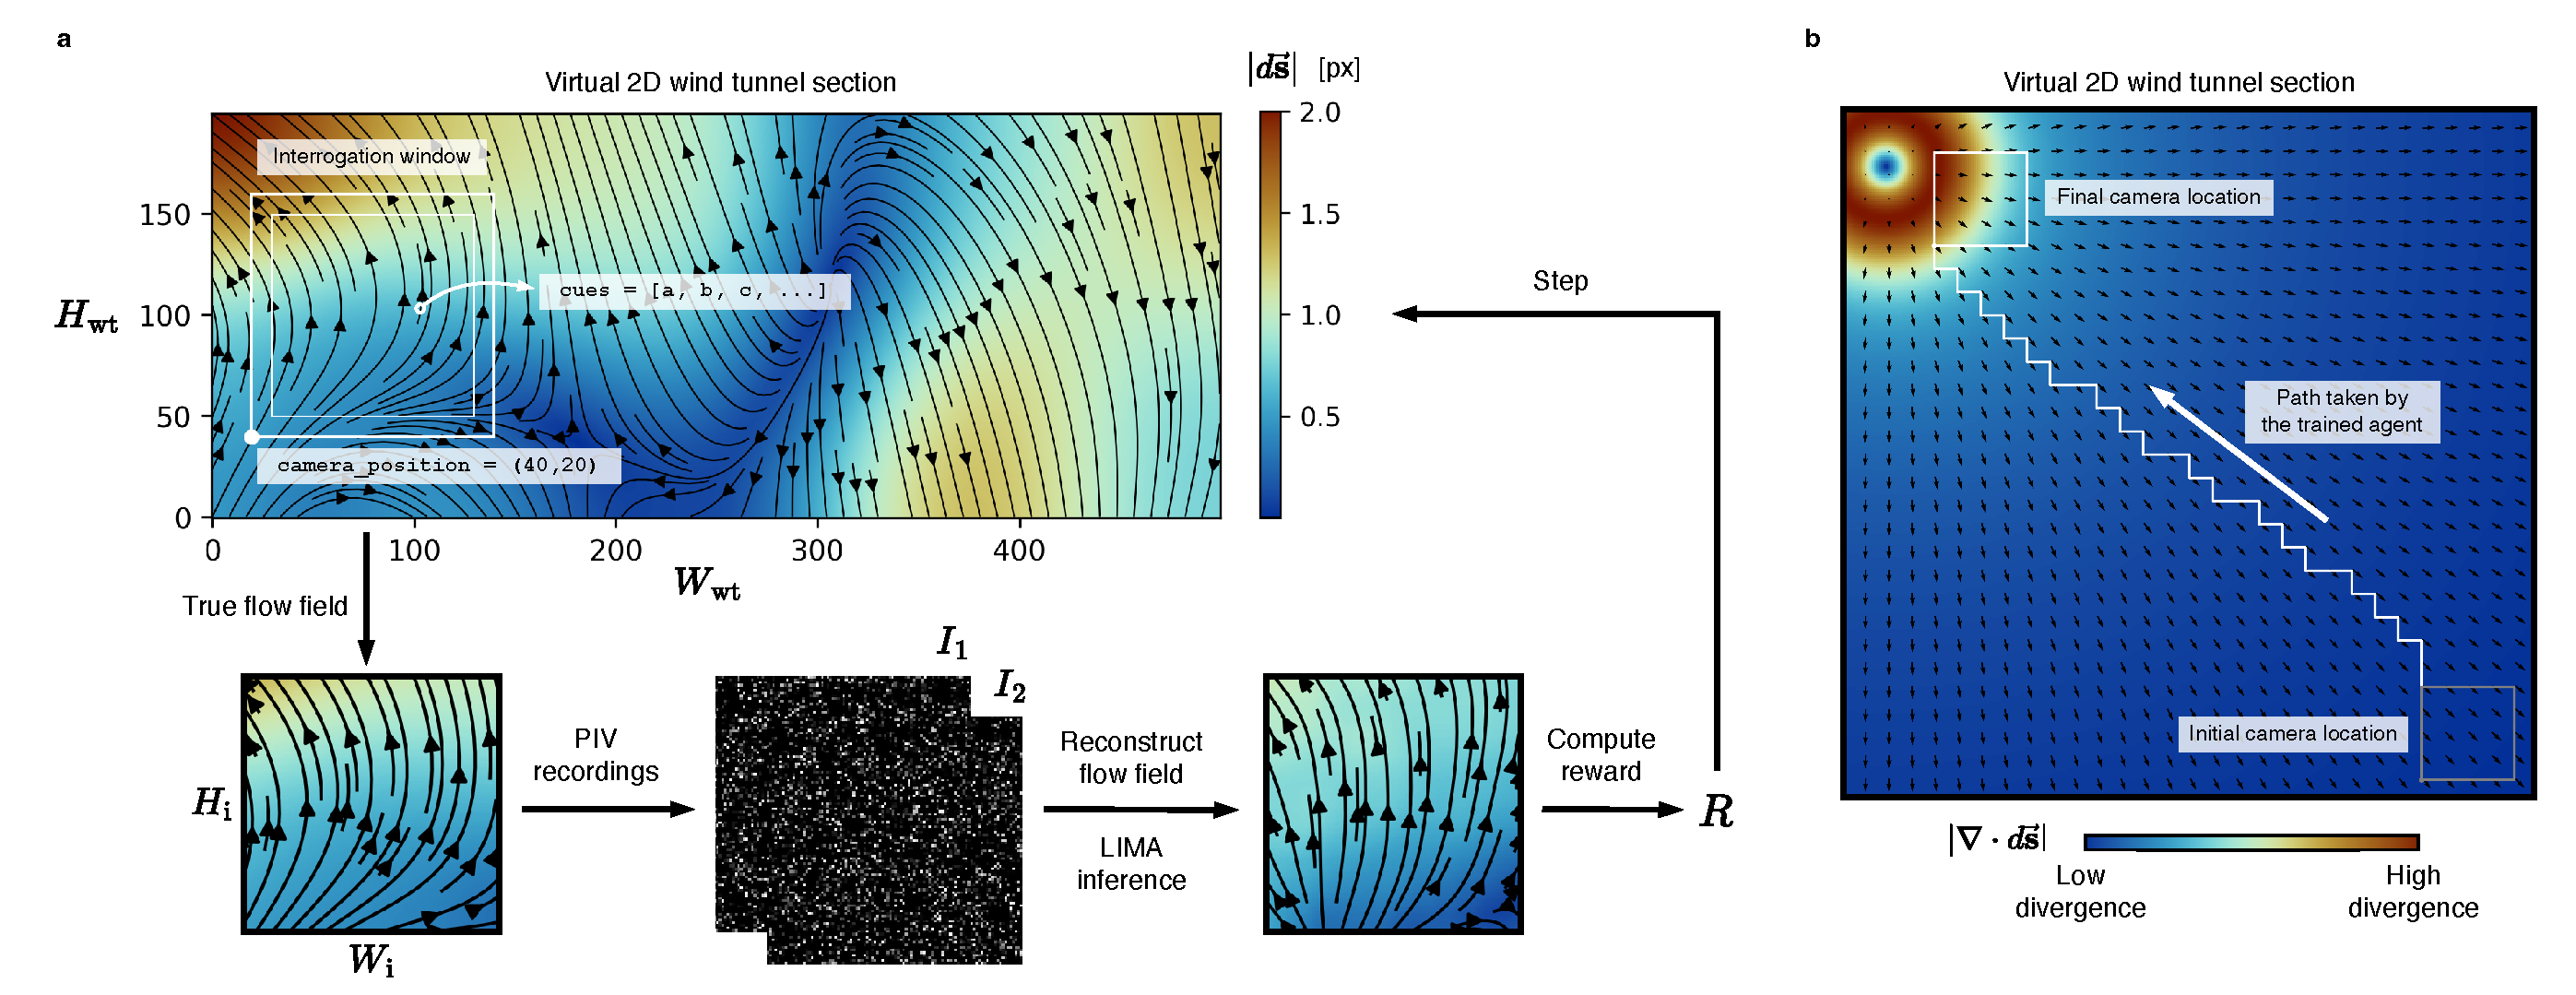
\includegraphics[width=\textwidth]{RL.pdf}
\vspace{10 pt}
\caption{\footnotesize (\textbf{a}) The setup used to training a reinforcement learning (RL) algorithm move a virtual camera and locate the source/sink in a radial flow. (\textbf{b}) Using the trained RL agent to change the camera position in a new environment.}
\label{fig:RL}
\end{figure*}

The virtual wind tunnel is modeled as a subclass of the Gymnasium environment \cite{brockman2016openai} using the dedicated \texttt{PIVEnv} class. A registered Gymnasium environment can be ported to RL libraries, such as TF-Agents \cite{TFAgents}. The basic structure of the PIV environment class is presented below:
\lstset{language=Python}
\begin{lstlisting}
import gymnasium as gym

class PIVEnv(gym.Env):

	def reset():

	def step():

	def render():

	def record_particles():

	def make_inference():

\end{lstlisting}
The functions \texttt{reset()}, \texttt{step()}, and \texttt{render()} are standard in most RL environments and allow to reset the environment to an initial state, make a step in the environment, and render the current state of the environment, respectively.
The function \texttt{record\_particles()} performs a ``virtual PIV'' at each step in the environment. The function \texttt{make\_inference()} allows to use a custom inference model (such as a CNN model) to predict flow targets from PIV recordings. 
Specific PIV parameters can be passed to the \texttt{PIVEnv} class through constructors: \\
\texttt{ParticleSpecs}, \texttt{FlowFieldSpecs}, \texttt{MotionSpecs}, and \texttt{ImageSpecs}. An example constructor for particle properties can be:
\lstset{language=Python}
\begin{lstlisting}
from pykitPIV import ParticleSpecs

particle_spec = {'diameters': (1, 4),
                 'densities': (0.05, 0.2),
                 'diameter_std': (0.1, 0.5),
                 'min_diameter': 0.1,
                 'seeding_mode': 'random',
                 'random_seed': 100}
                 
particle_spec = ParticleSpecs(particle_spec)
\end{lstlisting}
Fig.~\ref{fig:RL}b shows how the trained RL agent moves the camera by executing one of the five actions: move up, move down, move right, move left, stay. The final camera location is centered at a region of high divergence.

\section{Impact} \label{sec:results}

The kinematic training methodology \cite{manickathan2022kinematic} is the core concept behind generating PIV image pairs with \texttt{pykitPIV}, and has been used to train CNNs in optical flow estimation in the earlier works coming from our group \cite{manickathan2022kinematic, manickathan2023lightweight, mucignat2023lightweight}. 
Therefore, the core functionalities of \texttt{pykitPIV} are translated from the earlier MATLAB\copyright \, code used in our group.
The approach proved successful in training LIMA \cite{manickathan2022kinematic}, which suggests that for small enough $\Delta t$, learning the kinematic relationship between two consecutive PIV snapshots, as opposed to knowing the full dynamic relationship, is sufficient to train CNNs.

To date, we have been able to identify four openly-available synthetic image generation (SIG) packages: one written in the ANSI C language coming from the EUROPIV project \cite{lecordier2004europiv}, two written in MATLAB \citep{ben2020openpiv, mendes2020piv}, and third package, implemented in both MATLAB and Python, with a limited scope in order to specifically track defocusing and tackle astigmatic PIV. These existing SIG implementations make integrating with Python interfaces more difficult. With the emerging ML applications, a package that readily ports to libraries such as PyTorch \cite{paszke2017automatic, paszke2019pytorch}, TensorFlow \cite{tensorflow2015}, or Keras \cite{chollet2015keras} is the ideal solution. Moreover, ML algorithms for PIV are often trained using synthetic images generated with open-source realistic flowfields, \textit{e.g.}, taken from the John Hopkins Turbulence Database (JHTD) \cite{perlman2007data}. While the JHTD database is openly available, the synthetic image generation is often performed by different groups using in-house codes. We have hopes that providing \texttt{pykitPIV} as an open-source Python library, researchers can easily share their image generation workflows, making the training of ML algorithms fully reproducible.

% WHERE pykitPIV CAN HAVE IMPACT
We envision numerous areas where \texttt{pykitPIV} can have impact and can support the ongoing ML development for optical velocimetry. First, \texttt{pykitPIV} allows to generate training data for ML in a single Python workflow, but also allows the ML algorithm to interact with the image generation process. Specifically, the high flexibility in the types of created images can port very well with variational approaches or with RL algorithms, where an agent may learn to augment the training dataset in real-time to account for changes in experimental settings.
In addition to applications shown in \S\ref{sec:examples}, another recent application for CNNs is for learning location of particles for particle tracking velocimetry (PTV) \cite{godbersen2024peak}. There, \texttt{pykitPIV} could provide training datasets with known ground truth particle positions.
Another interesting path where \texttt{pykitPIV} can provide virtual environments is exploring unsupervised training of CNNs that does not require flow targets but is based on modified loss functions that look at photometric loss, constistency between image frames, and smoothness in the intensity fields \cite{lagemann2024challenges}. Our library can also integrate with the post-processing Python software developed in \cite{aguilar2022dpivsoft}. Finally, the powerful novelty of this package, as compared to previous MATLAB-based packages, is the introduction of new adjustable parameters that mimic various aspects of the experimental settings. The reader is referred to \href{https://pykitpiv.readthedocs.com}{software documentation} where we delineate many interesting examples for ML applications.

\section{Conclusions}

In this work, we present a Python library, \texttt{pykitPIV}, that acts as a ``virtual wind tunnel'', providing a playground for training and testing ML models for optical velocimetry. The richness of experimental conditions, reproducibility of training data generation, and ready-to-use integrations with PyTorch and TensorFlow can help advance the growing development of ML applications in experimental fluid dynamics. Currently, the main power lies in the specialized CNN architectures which can open avenues for real-time inference and interaction of trained ML models (such as RL) with the experiment. In fact, our group already uses LIMA in real-time for 15Hz PIV, but further improvements to inference speed are needed for higher image acquisition frequencies.
We therefore plan a continued development of this library. The future versions will include extension from 2D to 3D environments with the 3D PIV images generated using 2D camera projections. Future application can also include the use variational approaches to inform training data collection, or train a RL agent to construct necessary support data in new environments.

\section*{Declaration of competing interest}

The authors declare that they have no known competing financial interests or personal relationships that could have appeared to influence the work reported in this paper.

\section*{Author contributions}



\section*{Acknowledgments}



\bibliographystyle{pci}
\bibliography{bibliography}

\end{document}